\chapter{Design \& Specification}

This section will present an abstract view of how the system works.

\subsection{Use cases}
\begin{figure}[H]
  \centering

	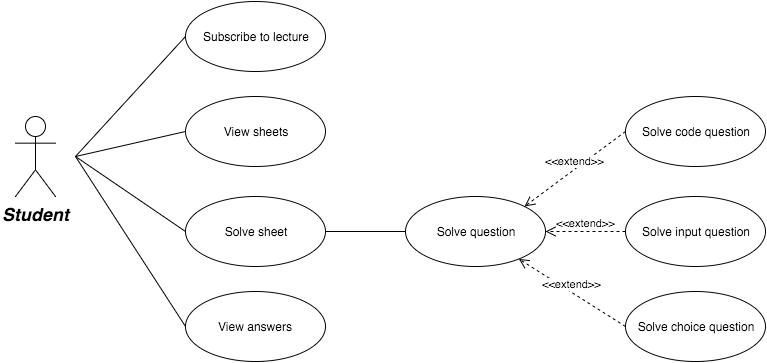
\includegraphics[width=\textwidth,height=\textheight,keepaspectratio]{cases}
	\caption{Use cases for students}
\end{figure}

\begin{figure}[H]
  \centering

	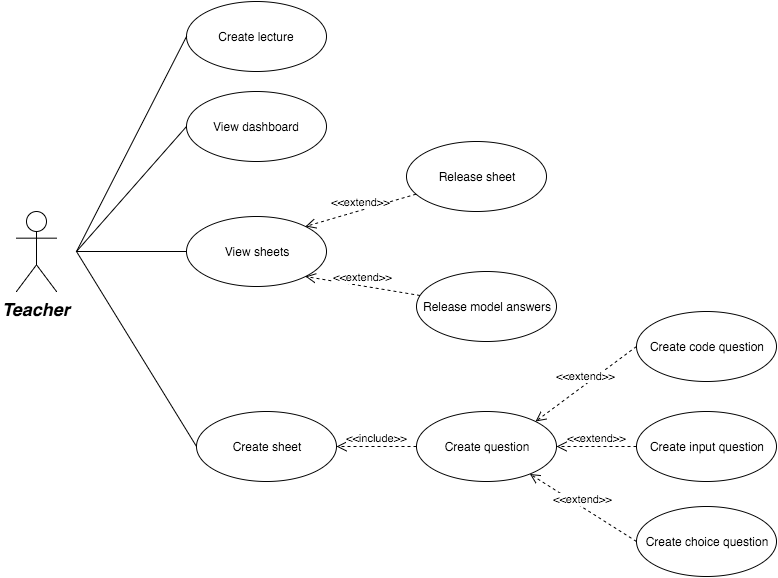
\includegraphics[width=\textwidth,height=\textheight,keepaspectratio]{cases2}
	\caption{Use cases for teachers}
\end{figure}

\subsection{System architecture}
\paragraph{User interface}
Since the user's are assumed to be somewhat technically savvy , the application takes some liberties with having a limited amount of help and information banners since it works similarly to other website the target audience is familiar with.
Overall the application is meant to have a flat design that looks good on any resolution.
Each lecture has a colour chosen by the teacher and shows up throughout the user interface so the user knows which lecture they are looking at.

\subsection{Third party libraries}

\subsubsection{React}
A javascript library that allows the project to have isolated , reusable components that build up all of the user interface

\subsubsection{Chromath} 
A javascript library that can manipulate colours. It is used within the dashboard to compute darker shades of the lecture color - this is useful for both the charts ( each section of the chart is a different colour ) and for the transition matrix ( the higher the transition count , the darker the shade ).

	It is statically included in the project.
	
\subsubsection{CodeMirror}
A javascript library that provides an embeddable code editor. Used to let user's write their own code.

\subsubsection{Markdown-it}
A javascript library used to render Markdown , in both the title preview on the sheet creation page and the actual sheet that the user sees.

\subsubsection{Highlight}
A javascript library to highlight code syntax , used internally by Markdown-it
	
\subsubsection{JQCloud}
A javascript library used to render a word cloud in the dashboard for input questions.

\subsubsection{Levenshtein-ffi}
A ruby gem that allows fast calculation of Levenshtein distances for answer's in the input question's dashboard.

\subsubsection{pg}
A ruby gem for Postgres support

\subsubsection{Devise}
A ruby gem that simplifies authentication

\subsubsection{ReactRails}
Support for React in Rails applications

\subsubsection{Typescript Rails}
Automatic compilation of typescript files as part of the rails asset pipeline.

